\documentclass{standalone}

\begin{document}


\section*{Computational Environments}\addcontentsline{toc}{section}{Computational Environments}
\markboth{Appendix F}{Computational Environments}

\begin{figure*}
\centering
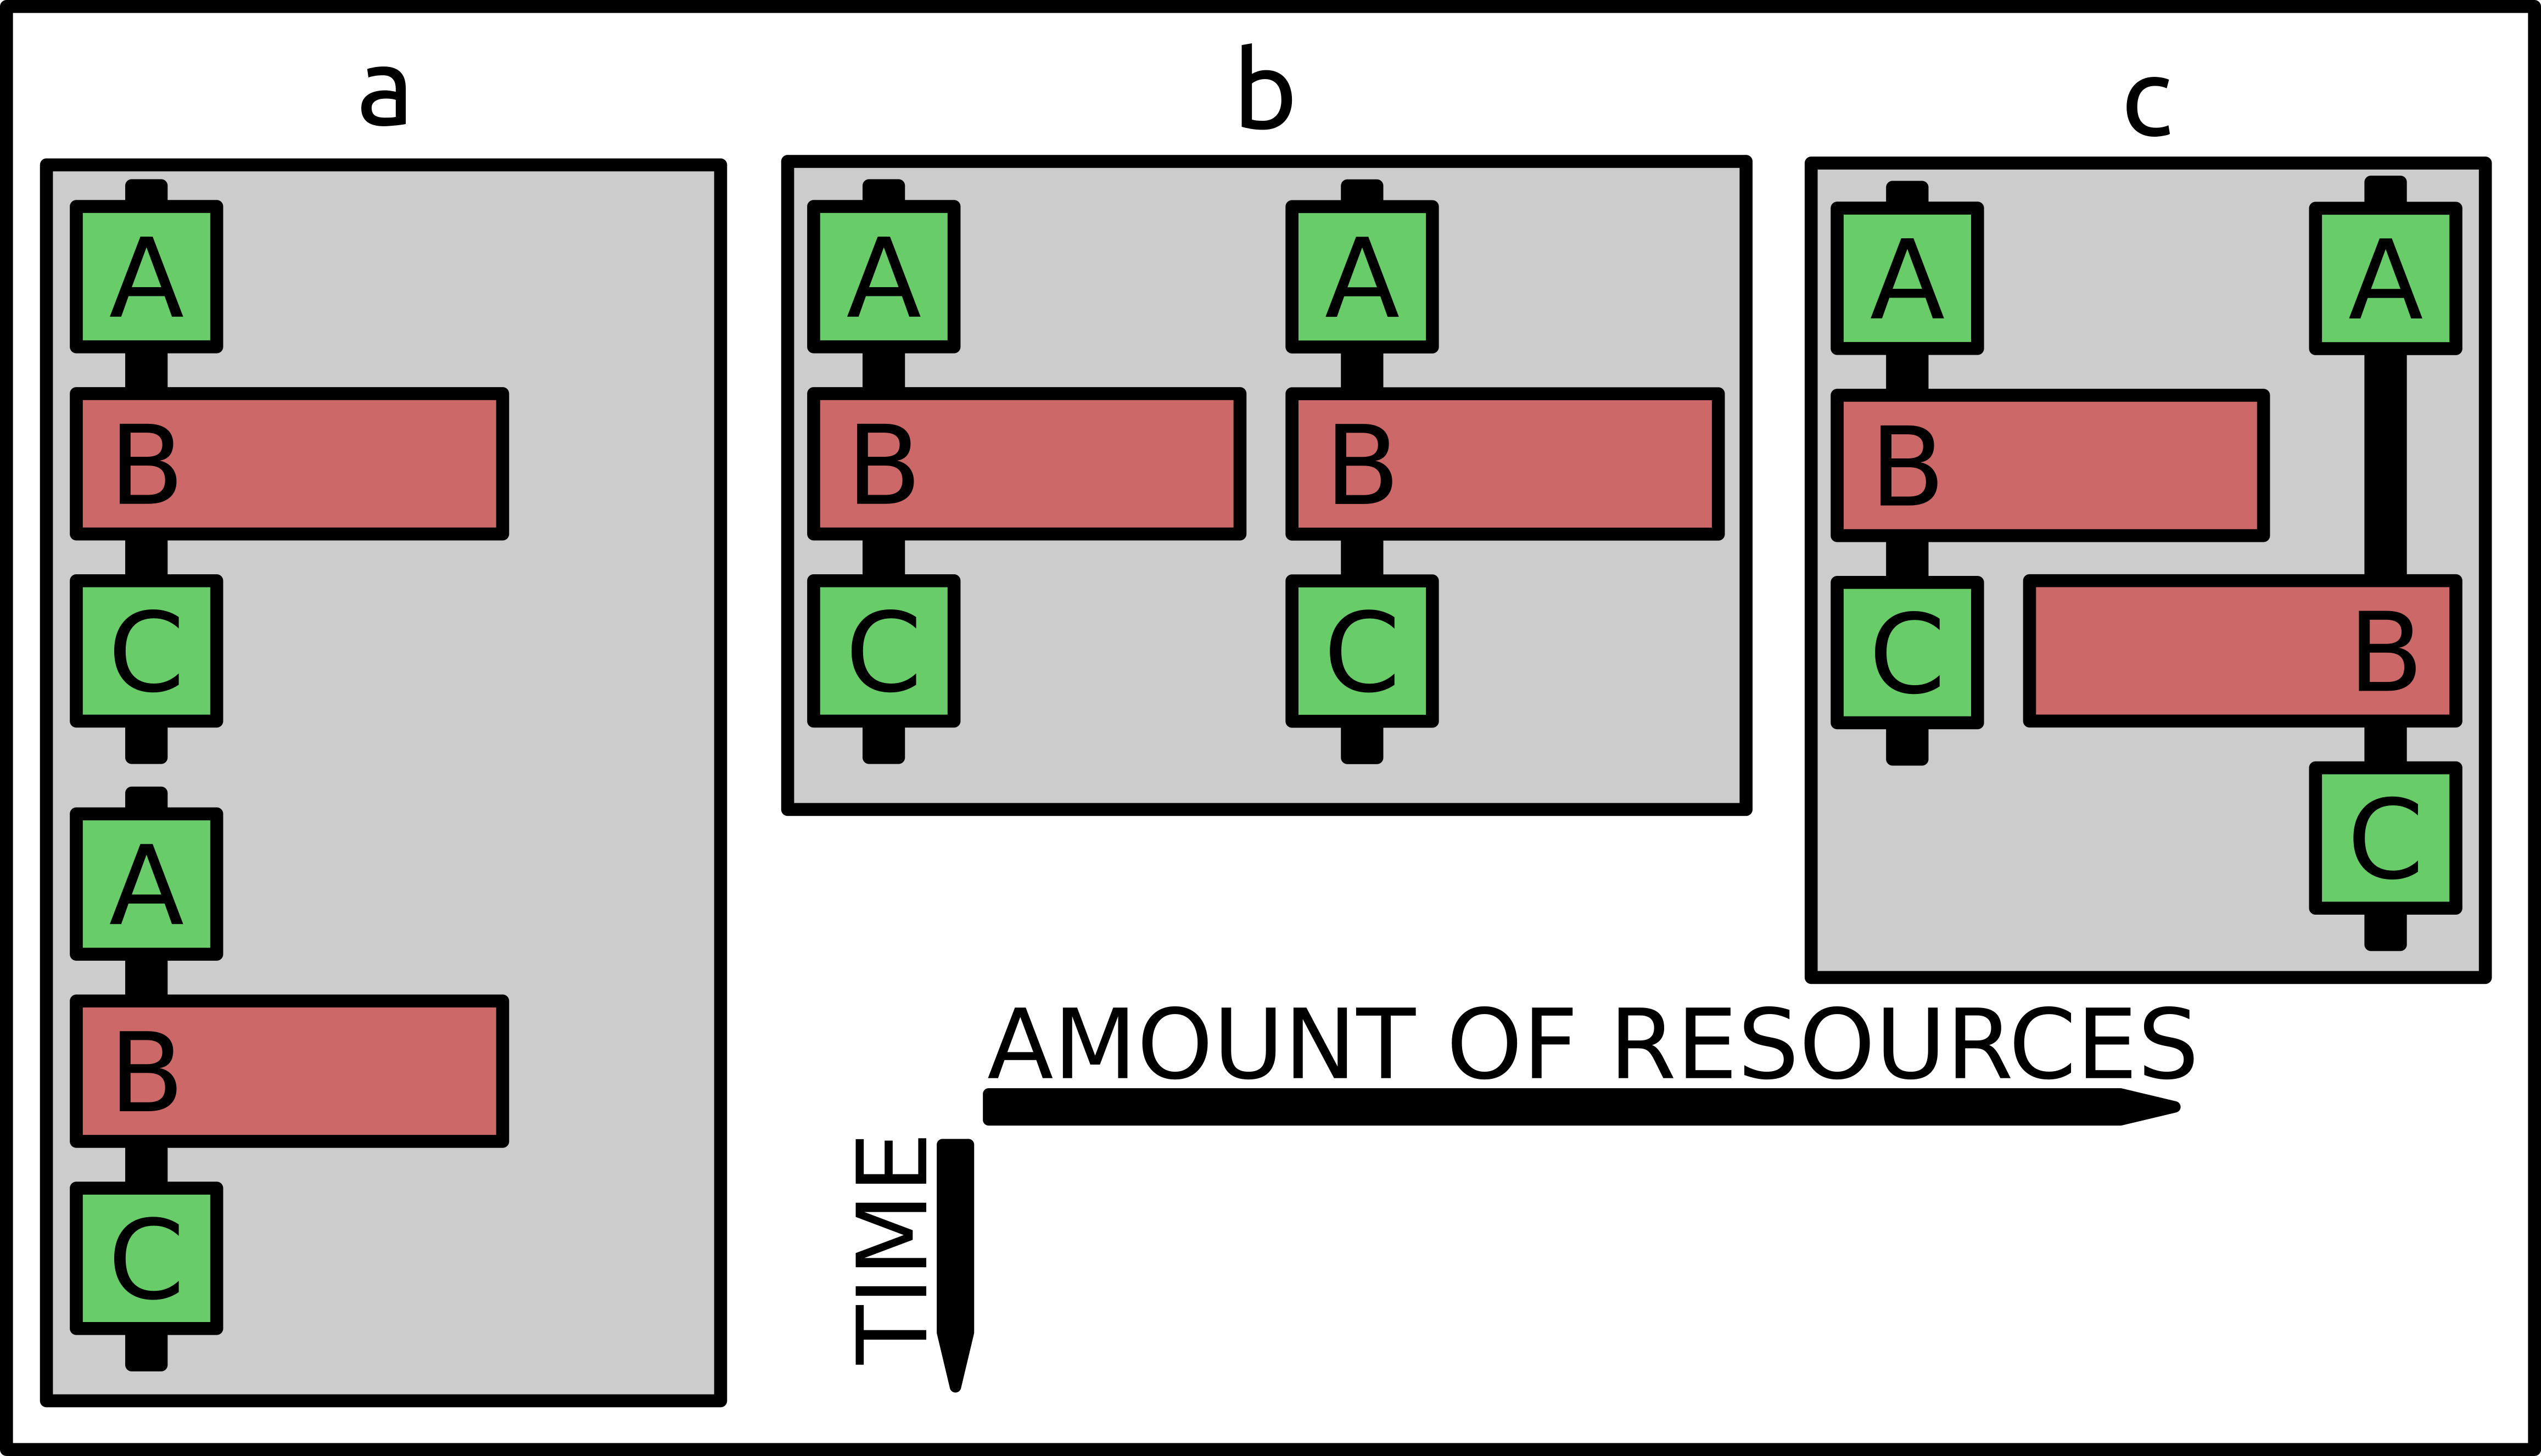
\includegraphics[width=.6\textwidth]{concurrency.png}
\caption{Examples of concurrency work-flow of two processes.
The first case ($a$) represents a simple (naive) sequential work-flow; the second ($b$) highlights a brute force parallelization; the third ($c$) is the case of a perfect match between the available resources and the requested resources.
Often brute force parallelization of pipelines done as in the image $b$ ends up overlapping the most computationally intensive steps.
Measuring the minimum viable requirements for the execution allow to better allocate resources as seen in the image $c$.}
\label{fig:wes_concurrency}
\end{figure*}

There are two main optimization strategies: the first is to improve the efficiency of a single run on a single patient and the second is to employ massive parallelization on various samples.
In both cases we have to know the necessary resources of the pipeline (and in a fine grain the resources of each step) and the optimal concurrency strategy to be applied to our work-flow (see Fig.~\ref{fig:wes_concurrency}).
In the analyses we want to highlight limits and efficiencies of the most common computational environments used in big data analytics, without any optimization strategy of the codes or systems.

We also focused on a single patient analysis, the base case study to design a possible parallelization strategy.
This is especially relevant for the multi-sample parallelization, that is the most promising of the two optimization strategies, as it does not rely on specific implementations of the softwares employed in the pipeline.

The pipeline was implemented on 5 computational environments: 1 server grade machine (Xeon E52640), 1 HPC node (Xeon E52683), 2 low power machines (Xeon D and Pentium J) and one virtual machine built on an AMD Opteron hypervisor.
The characteristics of each node are presented in Tab.~\ref{tab:node-characteristic}.

The server~-~grade node is a typical node used for bioinformatics computation, and as such features hundreds of GB of memory with multiple cores per motherboard: for these reasons we chose it as reference machine and the following results are expressed in relation to it.

The two low~-~power machines are designed to have a good cost~-~to~-~performance ratio, especially for the running cost\footnote{
  Running cost is evaluated as the energy consumption that the node requires per subject, assuming that the consumption scales linearly with the number of cores used in the individual step.
}.
These machines have been proven to be a viable solution for high performance computations~\cite{Cesini2017}.
Their low starting and running cost mean that a cluster of these machines would be more accessible for research groups looking forward to increase their computational power.

The last node is a virtual machine, designed to be operated in a cloud environment.

The monitoring tool used is \emph{Telegraf}, which is an agent written in Go for collecting, processing, aggregating, and writing metrics.
Each section of the pipeline sends messages to the \emph{Telegraf} daemon independently.

Regardless of the number of cores of each machine we restrict the number of cores used to only two to compare the statistics: this restriction certainly penalize the environment with multiple cores but with a view of maximizing the parallelizations and minimize the energy cost it is the playground to compare all the available environments.
Another restriction is applied to the chosen architectures: since available low~-~power machines provides only x86~-~architectures also the other environments are forced to work in x86 to allow the statistics comparison.

\begin{table*}
\hspace{-.75cm}
\begin{tabular}{llllll}
\hline \rowcolor{darkgrayrow}
\textbf{CLASS} & \multicolumn{2}{c}{\textbf{server grade machines}} & \multicolumn{2}{c}{\textbf{low power machines}} & \textbf{virtual machine}\\
\hline
\textbf{CPU}      & Intel Xeon  & Intel Xeon  & Intel Pentium & Intel Xeon  & AMD Opteron \\
\textbf{version}    & E5-2683v3   & E5-2640v2   & J4205   & D-1540  & 6386 SE   \\
\textbf{Microarchitecture}  & Haswell   & Ivy Bridge EP & Apollo Lake   & Broadwell   & Piledriver  \\
\textbf{Launch Date}    & Q3'14   & Q3'13   & Q4'16   & Q1'15   & Q3'12   \\
\textbf{Lithography}    & 22 nm   & 22 nm   & 14 nm   & 14 nm   & 32 nm   \\
\textbf{Cores/threads}    & 14/28   & 8/16    & 4/4     & 8/16    & 16    \\
\textbf{Base/Max Freq}    & 2.00/3.00   & 2.00/2.50   & 1.50/2.60   & 2.00/2.60   & 2.80/3.50 \\
\textbf{L2 Cache}     & 35 MB   & 20 MB   & 2 MB    & 12 MB   & 16 MB   \\
\textbf{TDP}      & 120 W   & 95 W    & 10 W    & 45 W    & 115 W   \\
\textbf{Total CPUs}     & 2     & 2     & 1     & 1     & 1   \\
\textbf{total cores/threads}  & 28/56   & 16/32   & 4/4     & 8/16    & 16    \\
\textbf{Total Memory}     & 256 GB  & 252 GB  & 8 GB    & 32 GB   & 60 GB   \\
\textbf{System power}     & 240 + 60 W  & 190 + 60 W  & 10 + 2 W  & 45 + 10 W   & 115 + 10 W  \\
\textbf{Electrical costs}   & 650 €/year  & 550 €/year  & 26 €/year   & 120 €/year  & 273€ /year  \\
\textbf{System price}   & 4000-6000 €   & 3000-5000 €   & 100-130 €   & 900-1200 €  & 2000-3000€  \\
\hline\\
\end{tabular}
\caption{Characteristics of the tested computational environments.
Electrical costs are estimated as 0.25~€/kWh; CPU frequencies are reported in GHz; TDP: Thermal Design Power, an estimation indicator of maximum amount of heat generated by a computer chip when a \quotes{real application} runs.}
\label{tab:node-characteristic}
\end{table*}

\end{document}
